La psychoacoustique est la branche de l'acoustique qui {\'e}tudie la
perception des sons par l'homme. Il s'agit donc d'{\'e}tudier les
relations entre les stimuli sonores et les sensations, voir
l'absence de sensations, qu'ils provoquent chez l'auditeur. Ainsi
il sera possible de simplifier un son de mani{\`e}re {\`a} ne garder que
ses composantes pertinentes, c'est {\`a} dire vraiment entendues par
l'oreille. Une telle simplification peut servir pour de la
compression audio (comme dans le standard MP3 par exemple), ou
bien comme cela nous int{\'e}resse pour la synth{\`e}se de son lorsque le
synth{\'e}tiseur a une puissance de calcul limit{\'e}e.\\

Il faut tout de m{\^e}me garder {\`a} l'esprit que la plupart des
r{\'e}sultats de la psychoacoustique ont {\'e}t{\'e} d{\'e}termin{\'e}s
exp{\'e}rimentalement. De plus, ces r{\'e}sultats sont valables pour un
auditeur moyen, c'est {\`a} dire un sujet n'ayant pas de probl{\`e}me
d'ou{\"\i}e, mais qui n'a pas non plus une acuit{\'e} auditive entra{\^\i}n{\'e}e.
En effet, les ph{\'e}nom{\`e}nes psychoacoustiques sont en grande partie
dus {\`a} la physiologie de l'oreille qui elle-m{\^e}me varie d'un sujet {\`a}
l'autre. Ainsi, une adaptation des r{\'e}sultats en fonction du sujet
cible peut {\^e}tre envisageable, par exemple l'utilisation des
concepts psychoacoustiques ne sera pas la m{\^e}me suivant que la
cible est constitu{\'e}e de personnes {\^a}g{\'e}es ou de musiciens
confirm{\'e}s.\\

Nous allons donc voir au cours de ce chapitre les quelques
principes th{\'e}oriques sur lesquels s'appuie la bo{\^\i}te {\`a} outils
d{\'e}velopp{\'e}e.\\


\newpage
\section{Courbes d'isosonie}
Courbes reliant la sensation de force du signal sonore sur
l'auditeur, exprim{\'e}e en sones, et l'intensit{\'e} acoustique r{\'e}elle,
mesur{\'e}e en d{\'e}cibels SPL \footnote{Le dB SPL (pour Sound Pressure
Level) quantifie l'intensit{\'e} acoustique d'un stimulus sonore. Il
est d{\'e}finie par $ I_{SPL} = 20 * \log _{10} \( \frac{P}{P_{0}} \)
$ o{\`u} $P_{0}$ repr{\'e}sente est la r{\'e}f{\'e}rence de 20 $\mu$ Pa. Ainsi un
niveau de 0 dB SPL correspond {\`a} un signal {\`a} la limite de l'audition {\`a} 1 kHz.}.\\

\begin{figure}[h]
    \bigskip
    \centering
    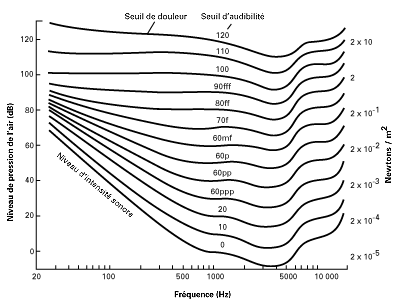
\includegraphics[width=12cm]{figures/isosonie.png}\\
    \caption{Courbes d'isosonie.}
    \label{isosonie}
    \bigskip
\end{figure}

Ces courbes, d{\'e}termin{\'e}es exp{\'e}rimentalement au cours des ann{\'e}es
trente \footnote{H. Fletcher et W. Munson, "Relation between
loudness and masking", \emph{J. Acoust. Soc. Amer.}, vol. 9, pp.
1-10, 1937.}, permettent d'{\'e}tablir la sensation de perception
{\'e}gale d'une intensit{\'e} acoustique donn{\'e}e, et cela pour l'ensemble
du spectre fr{\'e}quentiel audible. Elles sont extr{\^e}mement utiles
lorsqu'il s'agit de d{\'e}terminer les r{\'e}gions spectrales
significatives sur le plan perceptif lors d'op{\'e}rations d'encodage
et de compression de signaux audio-num{\'e}riques.\\

En particulier, la courbe du seuil absolue d'audition se place
pour des signaux sonores {\`a} la limite de la sensation de
perception. Une approximation possible \footnote{E. Terhardt,
"Calculating virtual pitch", \emph{Hearing res.}, vol. 1, pp.
155-182, 1979.} de ce seuil en fonction de la fr{\'e}quence est :
$$ S(f) = 3.64*f^{-0.8} - 6.5*e^{-0.6*(f-3.3)^{2}} + 10^{-3}*f^{4} $$
o{\`u} f est en kHz et S en dB SPL.


\newpage
\section{Bandes critiques}
Pour une fr{\'e}quence centrale donn{\'e}e, la bande critique est la plus
petite largeur spectrale pour laquelle une m{\^e}me zone de la
membrane basilaire est excit{\'e}e. En effet, lorsque une onde sonore
arrive au pavillon de l'oreille, elle est transmise par la cha{\^\i}ne
des osselets (non repr{\'e}sent{\'e}e figure \ref{cochlee}) {\`a} l'oreille
interne. Cette derni{\`e}re se compose essentiellement de la cochl{\'e}e
(ou lima\c{c}on en raison de sa forme). Celle-ci est constitu{\'e}e de
deux canaux, les rampes vestibulaire et tympanique, s{\'e}par{\'e}s par la
la cloison cochl{\'e}aire. Cette cloison comprend la membrane de
Reissner, la membrane tectoriale, la membrane basilaire ainsi que
l'organe de Cortie pris entre ces deux derni{\`e}res. La vibration
sonore engendre des ventres d'onde le long de la membrane
basilaire {\`a} des positions sp{\'e}cifiques de sa fr{\'e}quence. Or l'organe
de Cortie qui repose sur la membrane basilaire, est constitu{\'e}e de
cellules cili{\'e}es au contact desquelles prennent naissance les
fibres du nerf auditif.\\

\begin{figure}[h]
    \bigskip
    \centering
    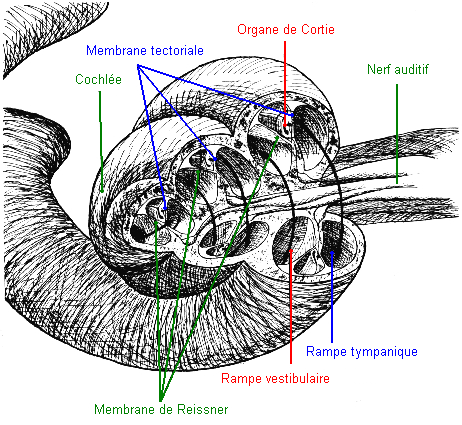
\includegraphics[width=12cm]{figures/cochlee.png}\\
    \caption{Coupe de la cochl{\'e}e.}
    \label{cochlee}
    \bigskip
\end{figure}

C'est l'espacement de ces cellules cili{\'e}es le long de la membrane
basilaire qui engendre le ph{\'e}nom{\`e}ne des bandes critiques. En effet
chaque r{\'e}cepteur nerveux se trouve accord{\'e} {\`a} une certaine
fr{\'e}quence due {\`a} sa position sur la membrane basilaire. Ainsi,
l'oreille effectue une transformation fr{\'e}quences/positions, et
c'est bien une information de position qui est transmise au
cerveau par le nerf auditif.\\

En cons{\'e}quence d'une telle transformation, le fonctionnement de
l'oreille interne s'apparente {\`a} celui d'un banc de filtres
passe-bandes {\`a} fort taux de recouvrement \footnote{i.e. les bandes
passantes des filtres se chevauchent.}, de plus la r{\'e}ponse en
fr{\'e}quence de chacun de ces filtres est asym{\'e}trique et leur
bande-passante d{\'e}pend de la fr{\'e}quence centrale \footnote{D. D.
Greenwood, "Critical bandwith and the frequency coordinates of the
basilar membrane", \emph{J. Acoust. Soc. Amer.}, pp. 1344-1356,
Oct. 1961.}, la bande-critique correspondrait {\`a} la largeur de la
bande-passante. En cons{\'e}quence, si deux fr{\'e}quences pures
appartenant {\`a} la m{\^e}me bande critique se pr{\'e}sentent au m{\^e}me instant
{\`a} l'oreille, il est possible que l'auditeur n'en per\c{c}oive qu'une.
Ainsi, une {\'e}chelle des fr{\'e}quences rendant compte de ces ph{\'e}nom{\`e}nes
a {\'e}t{\'e} invent{\'e}e, le Bark, et elle sera utilis{\'e}e avantageusement {\`a}
la place de l'{\'e}chelle de Hertz lorsqu'il est question de
perception humaine de signaux sonores. Un bark est d{\'e}fini comme la
largeur d'une bande critique, donc dans l'{\'e}chelle
de Bark les filtres sont de bande-passante constante.\\

\begin{figure}[h]
\bigskip
\begin{center}
    \begin{tabular}{|c|c||c|c||c|c|}
        \hline
        Bark &   Hertz   &   Bark    &   Hertz   &   Bark    &   Hertz\\
        \hline
        1    &   101     &   9       &   1079    &   17      &   3822\\
        2    &   204     &   10      &   1255    &   18      &   4554\\
        3    &   308     &   11      &   1456    &   19      &   5411\\
        4    &   417     &   12      &   1690    &   20      &   6414\\
        5    &   530     &   13      &   1968    &   21      &   7617\\
        6    &   651     &   14      &   2302    &   22      &   9166\\
        7    &   781     &   15      &   2711    &   23      &   11414\\
        8    &   922     &   16      &   3211    &   24      &   15405\\
        \hline
    \end{tabular}
\end{center}
\caption{Equivalence Bark/Hertz.}
\label{tabbark2hz}
\bigskip
\end{figure}

Pour un auditeur moyen, la largeur (en Hz) de bande critique en
fonction de la fr{\'e}quence centrale peut {\^e}tre estim{\'e}e par :
$$ BP_{crit}(f) = 25 + 75*\[ 1 + 1.4*\( \frac{f}{1000} \)^{2} \]^{0.69} $$
de plus, la formule :
$$ B(f) = 13 * \arctan\(7.6*10^{-4}*f\) + 3.5*\arctan\[\(\frac{f}{7500}\)^{2}\]$$
est souvent utilis{\'e}e pour convertir les Hertz en Bark
\footnote{Ces deux formules sont tir{\'e}es de: E. Zwicker et H.
Fastl, "Psychoacoustics facts en models", 1990.}.


\newpage
\section{Masquage fr{\'e}quentiel}
On parle de masquage lorsque une composante sonore est rendue
inaudible {\`a} cause de la pr{\'e}sence d'une autre composante. Le
masquage fr{\'e}quentiel, ou masquage simultan{\'e}, peut arriver lorsque
deux stimuli sonores ou plus sont pr{\'e}sent{\'e}s au syst{\`e}me auditif.
Plus pr{\'e}cis{\'e}ment, un signal sonore puissant peut engendrer une
excitation de la membrane basilaire suffisamment forte pour
emp{\^e}cher l'audition d'un signal plus faible situ{\'e} dans la m{\^e}me
bande critique. Malgr{\'e} le fait que les spectres de signaux audios
r{\'e}els peuvent g{\'e}n{\'e}rer une infinit{\'e} de scenarii de masquage
diff{\'e}rents, il est commun de s{\'e}parer ce ph{\'e}nom{\`e}ne en trois
probl{\`e}mes distincts et g{\'e}n{\'e}riques, facilitant ainsi son
exploitation dans des algorithmes audio-num{\'e}riques.\\

    \newpage
    \subsection{Masquage d'un ton par un autre ton}

    \begin{figure}[h]
        \centering
        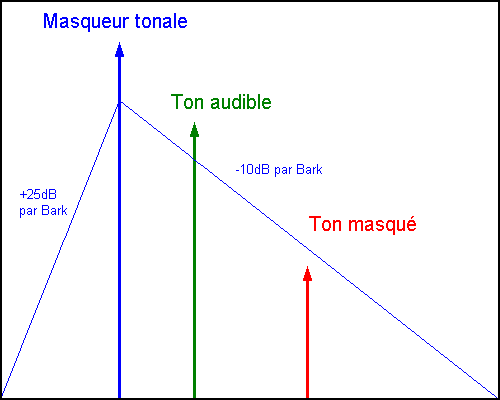
\includegraphics[width=12cm]{figures/masquage_tt.png}\\
        \caption{Ton masqu{\'e} par un ton.}
        \label{masquage_tt}
    \end{figure}

    Dans le cas d'interaction de deux signaux purement sinuso{\"\i}daux,
    on consid{\'e}rera qu'un ton est inaudible si il est situ{\'e} en
    dessous de la courbe de masquage (cf figure \ref{masquage_tt})
    induite par la fr{\'e}quence ayant localement le plus d'{\'e}nergie.
    Il est {\`a} noter que cette courbe ne s'{\'e}tale pas uniquement sur
    la bande critique de la fr{\'e}quence consid{\'e}r{\'e}e.


    \newpage
    \subsection{Masquage d'un ton par un bruit}
    Il peut arriver qu'un ton soit masqu{\'e} par le bruit de fond
    situ{\'e} dans la m{\^e}me bande critique. Cela arrive lorsque
    l'{\'e}nergie moyenne de la bande critique consid{\'e}r{\'e}e est
    sup{\'e}rieure d'au moins 4 dB {\`a} l'{\'e}nergie du signal sinuso{\"\i}dal.
    Une {\'e}tude de ce ph{\'e}nom{\`e}ne pourra {\^e}tre trouv{\'e}e dans [R.
    Hellman, "Assymetry of maskink between noise and tone",
    Percept. Psychphys, vol. 11, pp. 241-246, 1972].

    \begin{figure}[h]
        \centering
        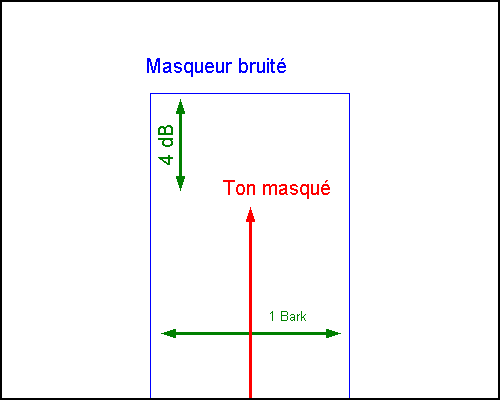
\includegraphics[width=12cm]{figures/masquage_tb.png}\\
        \caption{Ton masqu{\'e} par une bande de bruit.}
        \label{masquage_tb}
    \end{figure}


    \newpage
    \subsection{Masquage d'un bruit par un ton}
    La situation inverse est {\'e}galement possible. C'est {\`a} dire
    qu'un ton masquera le bruit de fond de sa bande critique si
    l'{\'e}nergie du signal pure est sup{\'e}rieure d'au moins 24 dB {\`a}
    l'{\'e}nergie moyenne de la bande critique consid{\'e}r{\'e}e. Une {\'e}tude
    compl{\`e}te de ce cas ainsi que du cas o{\`u} un ton masque un autre
    ton pourra {\^e}tre trouv{\'e}e dans [B. C. J. Moore, J. I.
    Alc\'{a}ntara et T. Dau, "Masking patterns for sinusoidal and
    narrow-band noise maskers", \emph{J. Acoust. Soc. Amer.}, vol.
    104, no. 2.1, pp 1023-1038, jan. 1998].\\

    \begin{figure}[h]
        \centering
        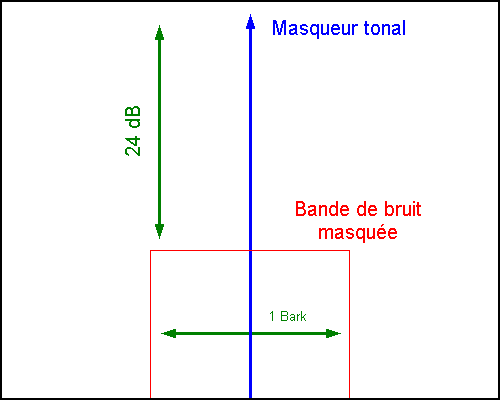
\includegraphics[width=12cm]{figures/masquage_bt.png}\\
        \caption{Bande de bruit masqu{\'e}e par un ton.}
        \label{masquage_bt}
    \end{figure}

    On remarque une dissym{\'e}trie entre ces deux derniers
    ph{\'e}nom{\`e}nes. Elle rend compte du fait que l'oreille humaine
    distingue plus facilement un signal sinuso{\"\i}dal noy{\'e} dans du
    bruit que l'inverse.
